\documentclass[12pt]{article}
\usepackage{array}
\usepackage{amsmath}
\usepackage{mathtools}
\usepackage{gensymb}
\usepackage{graphicx}
\usepackage{float}
\usepackage{caption}
\usepackage{setspace}
\usepackage[margin=0.75in]{geometry}

\newcommand{\cel}{\mathrm{\degree C}}

\allowdisplaybreaks

\begin{document}

    \title{The Specific Heat of Three Unknown Metals}
    \author{Ryan Coyne, Ben Eid, Erin Snook}
    \maketitle

    \section{Abstract}
        The specific heat capacity of three unknown metals was measured using a calorimeter. They were measured to be \(453 \pm 10 ~\mathrm{J/(kg\cdot K)}\), \(886 \pm 50 ~\mathrm{J/(kg\cdot K)}\), and \(289 \pm 12 ~\mathrm{J/(kg\cdot K)}\).
    \section{Introduction}
        Specific heat is the property of a substance which represents the energy requirement of raising its temperature. It may not seem intuitive that the energy required to raise the temperature by a particular amount would differ from one substance to another, but it is the case. Specific heat differs between substances in large part because of the differences in degrees of freedom, or the number of ways that molecule can move, rotate, or vibrate, that their constituents have. This is based on the equipartition theorem which states that a molecule's thermal energy is distributed evenly among its degrees of freedom. For example a monatomic gas has three degrees of freedom because the atoms can move in any combination of three dimensions but has no meaningful rotation, and there is no vibration because there are no bonds which can vibrate. 

        In contrast, a diatomic gas has up to six degrees of freedom. It still has the same three translational degrees of freedom as the monatomic gas, but it can also rotate around two axes and vibrate along its single bond. Water, is one substance that breaks from this degrees of freedom rule, with its specific heat being much higher than the equipartition theorem would otherwise predict. This break from the rule is largely due to the hydrogen bonding between water molecules which can store energy by being broken when heat is added to the water. 
    \section{Procedure}
        First set out one large bowl, one calorimeter, one triple beam balance, one hot plate, a plastic bag, a pot, two computer connected thermometers, and three metal objects, each of which are made of a single but different metal. Fill the bowl with ice. Fill the pot with water, set it on the hot plate, and turn on the hot plate. Place one of the metal objects in the plastic bag and then place the bag in the bowl of ice so that the object is completely covered with ice. Measure the mass of the inner cup of the calorimeter, and each metal object using the triple beam balance. Place one thermometer in the ice and one in the pot of water that is on the hot plate. Begin recording the temperatures of each. Allow the pot of water to heat up and adjust the temperature of the hot plate as needed until the water has reached equilibrium around 50\(\cel\).

        Next, stop recording the temperature of the pot and fill the inner cup of the calorimeter with hot water from the pot and perform the following steps quickly so that it loses the least amount of heat possible. Measure its mass once on the triple beam balance. Move the thermometer from the pot to the inner cup of the calorimeter. Place the inner cup of the calorimeter inside the outer cup. Begin recording the temperature. Remove the metal object from the bag and place it into the water in the calorimeter. Wait for the temperature of the calorimeter system to reach equilibrium and then wait for a few seconds to allow for enough data to create a linear fit from and stop recording. Repeat for the other two metal objects.

        \begin{figure}[H]
            \centering
            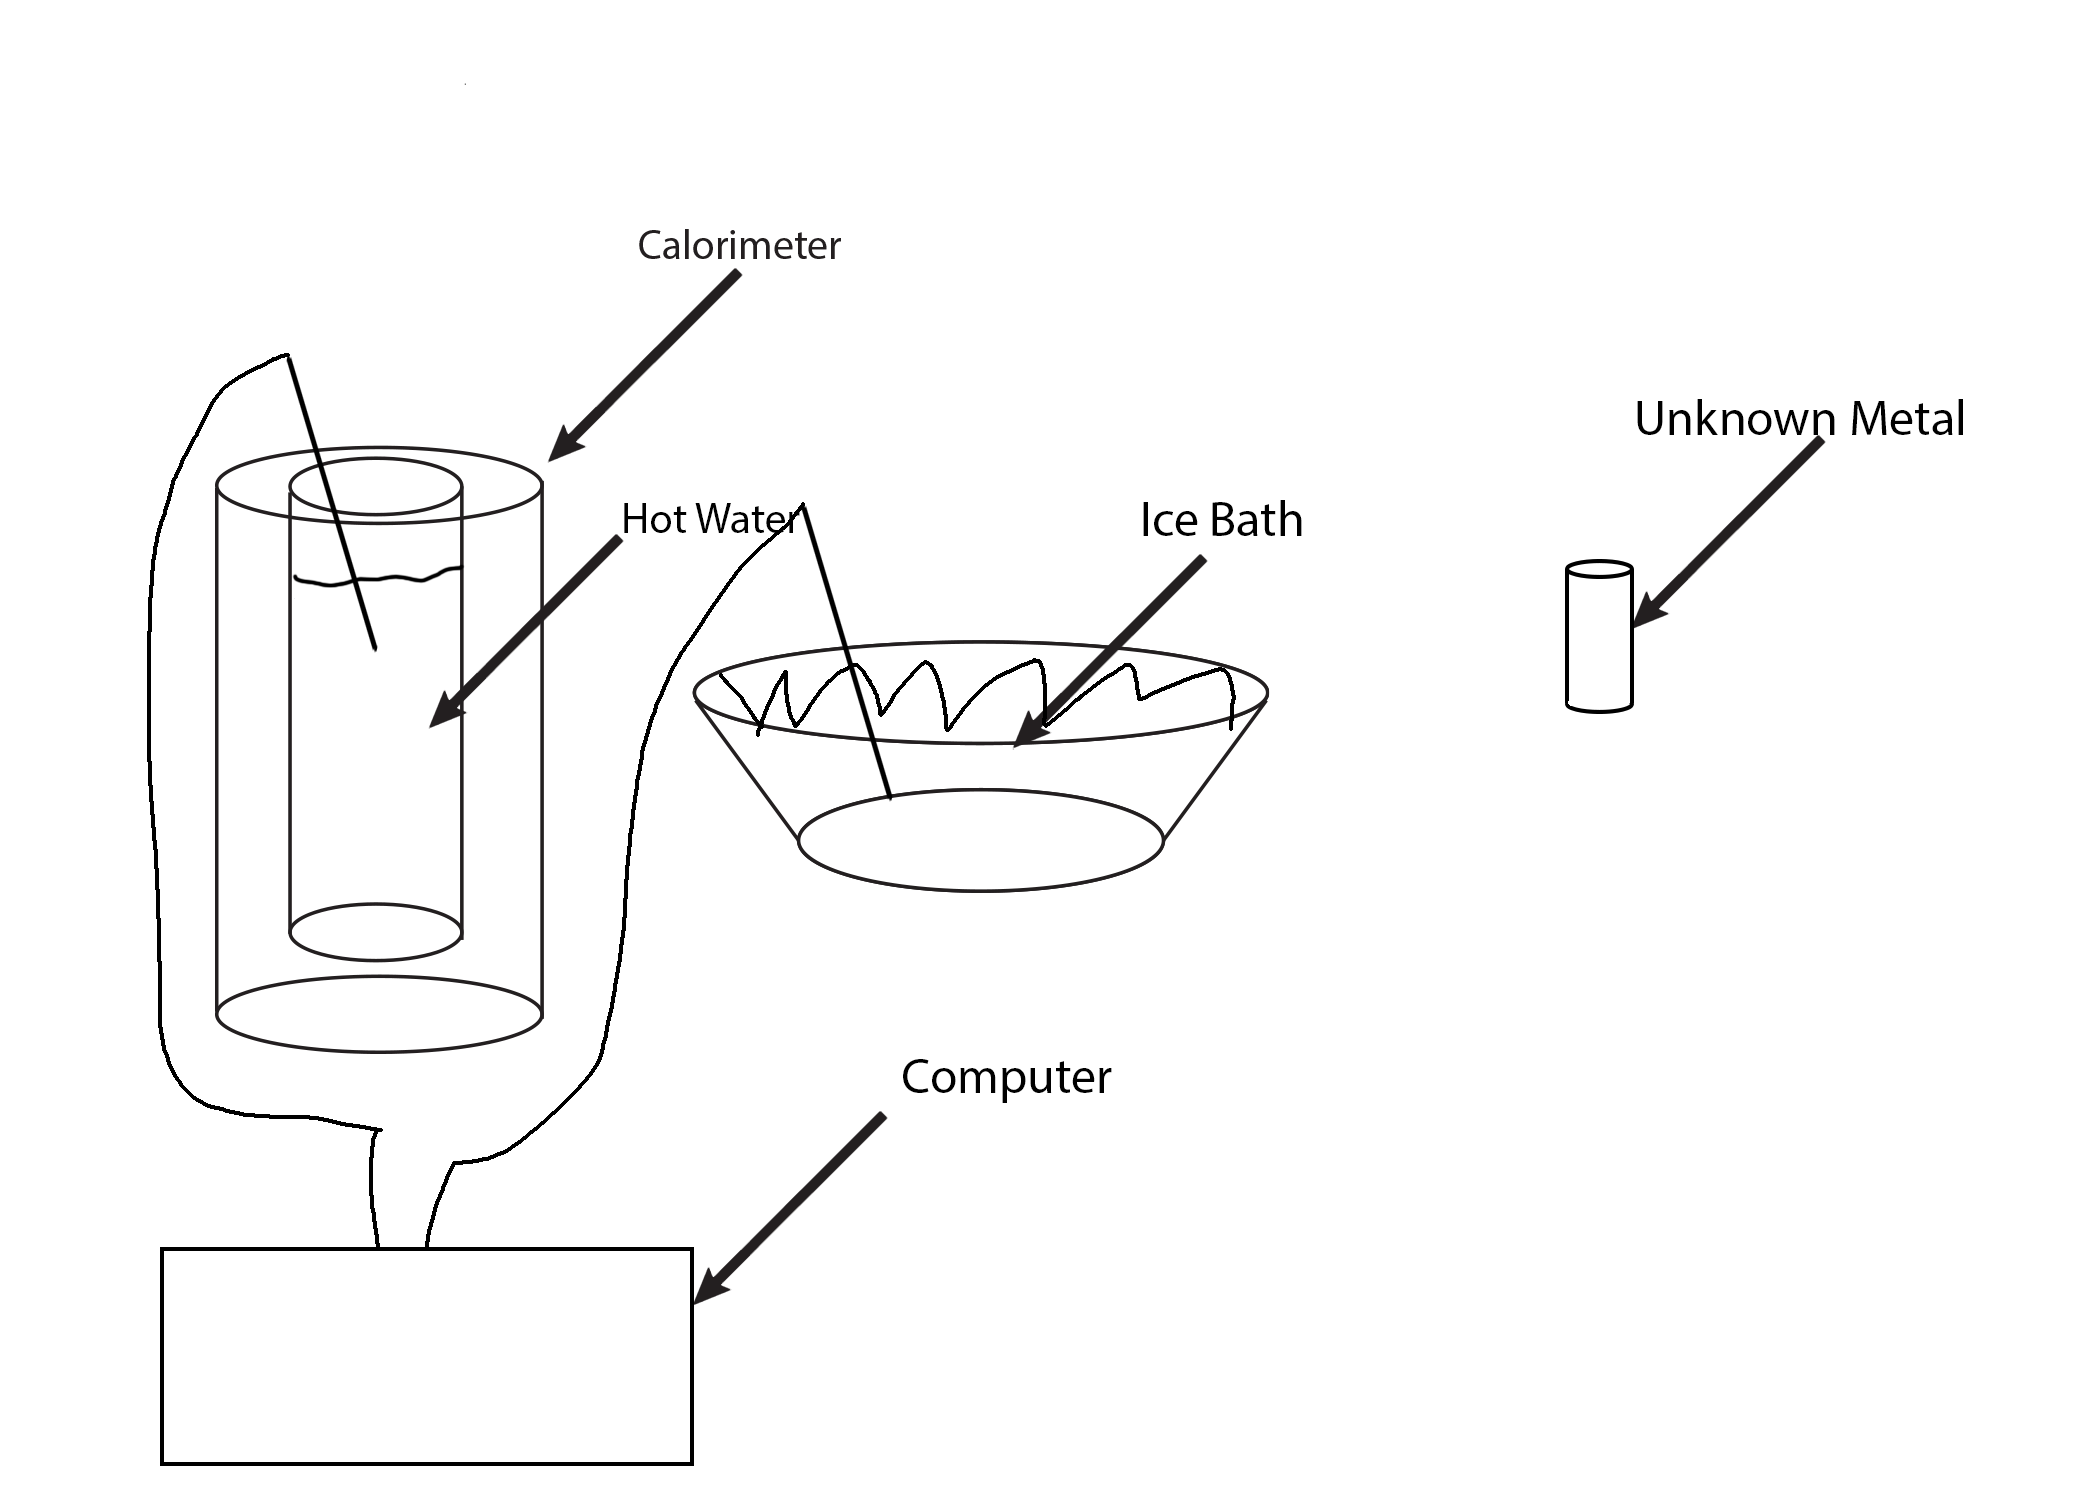
\includegraphics[width=0.9\linewidth]{setup.png}
            \caption{Experimental setup.}
        \end{figure}
    \section{Data}
        \begin{center}
            \begin{tabular}{c|c}
                 & \(m_c\) (g) \\
                \hline
                1 & 24.75 \\
                2 & 24.85 \\
                3 & 24.81 \\
                \hline
                \(\overline{x}\) & 24.787 \\
                \(\sigma_x\) & 0.078 
            \end{tabular}\\[6pt]
                Table 1: Mass of inner cup.\\[12pt]
            \begin{tabular}{c|c|c|c}
                 &\(M_1\) (g) & \(M_2\) (g) & \(M_3\) (g)\\
                \hline
                1 & 53.85 & 17.68 & 48.95\\
                2 & 53.89 & 17.83 & 49.01\\
                3 & 53.83 & 17.89 & 48.89\\
                \hline
                \(\overline{x}\) & 53.857 & 17.80 & 48.950\\
                \(\sigma_x\) & 0.031 & 0.11 & 0.060
            \end{tabular}\\[6pt]
            Table 2: Masses of the unknown metals.\\[12pt]

            \begin{tabular}{c|c|c|c|c|c}
                & \(m_w\) (g) &\(T_{wi}\) (\(\mathrm{\degree C}\)) & \(T_{mi}\) (\(\mathrm{\degree C}\)) & \(T_{fH}\)  (\(\mathrm{\degree C}\)) & \(T_{fL}\) (\(\mathrm{\degree C}\))\\
                \hline
                1 & 57.25 & 0.0556 & 48.8 & 44.76 & 44.55\\
                2 & 56.20 & 0.0970 & 45.9 & 43.42 & 43.11\\
                3 & 53.49 & 0.104 & 44.9 & 42.58 & 42.37\\
            \end{tabular}\\[6pt]
            Table 3: Mass of the water and temperature of the water, metal and the system at equilibrium.
        \end{center}
        \begin{figure}[H]
            \centering
            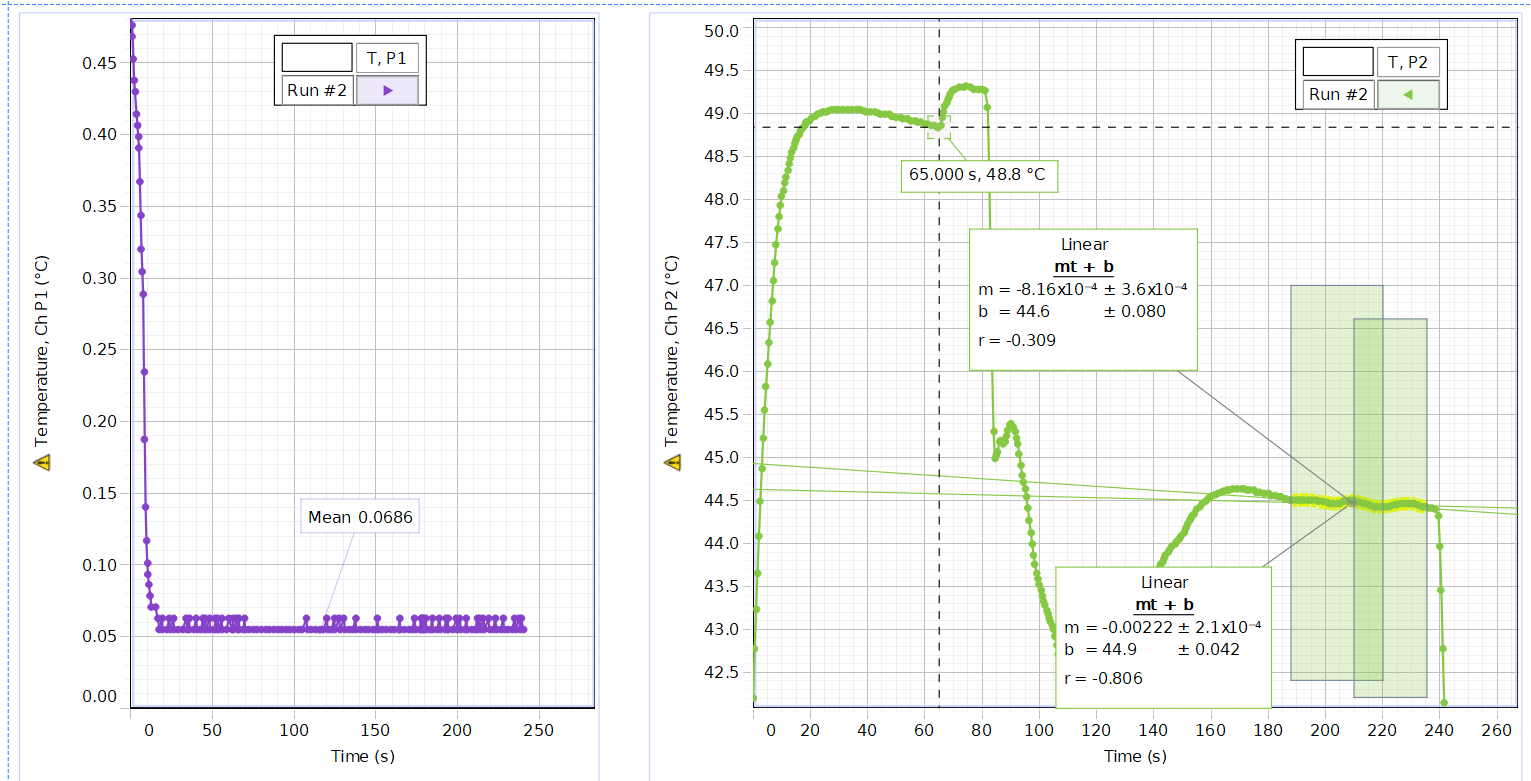
\includegraphics[width=0.9\linewidth]{f1.png}
            \caption{Plot of \(T\) vs \(t\) for metal 1.}
        \end{figure}
        \begin{figure}[H]
            \centering
            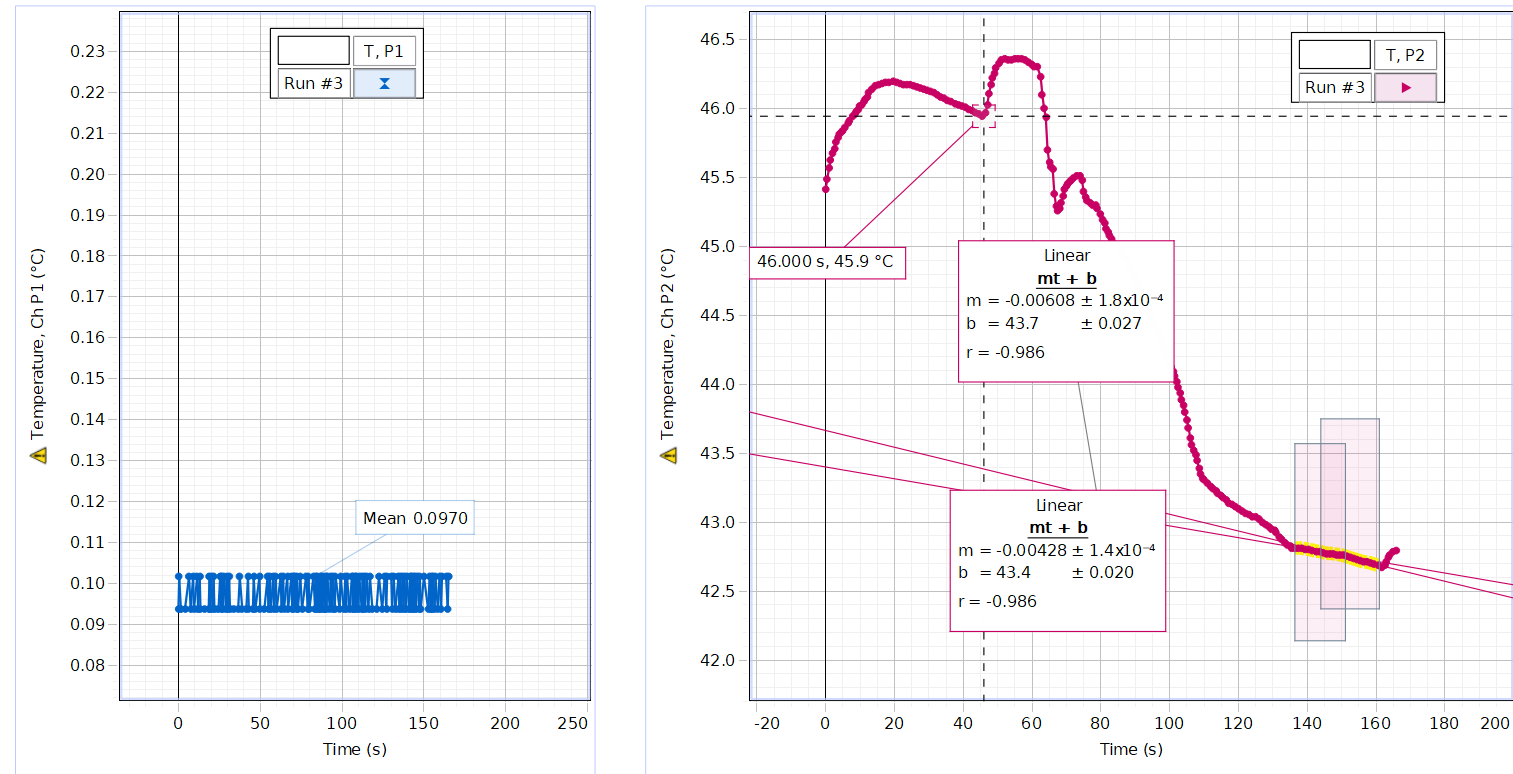
\includegraphics[width=0.9\linewidth]{f2.png}
            \caption{Plot of \(T\) vs \(t\) for metal 2.}
        \end{figure}
        \begin{figure}[H]
            \centering
            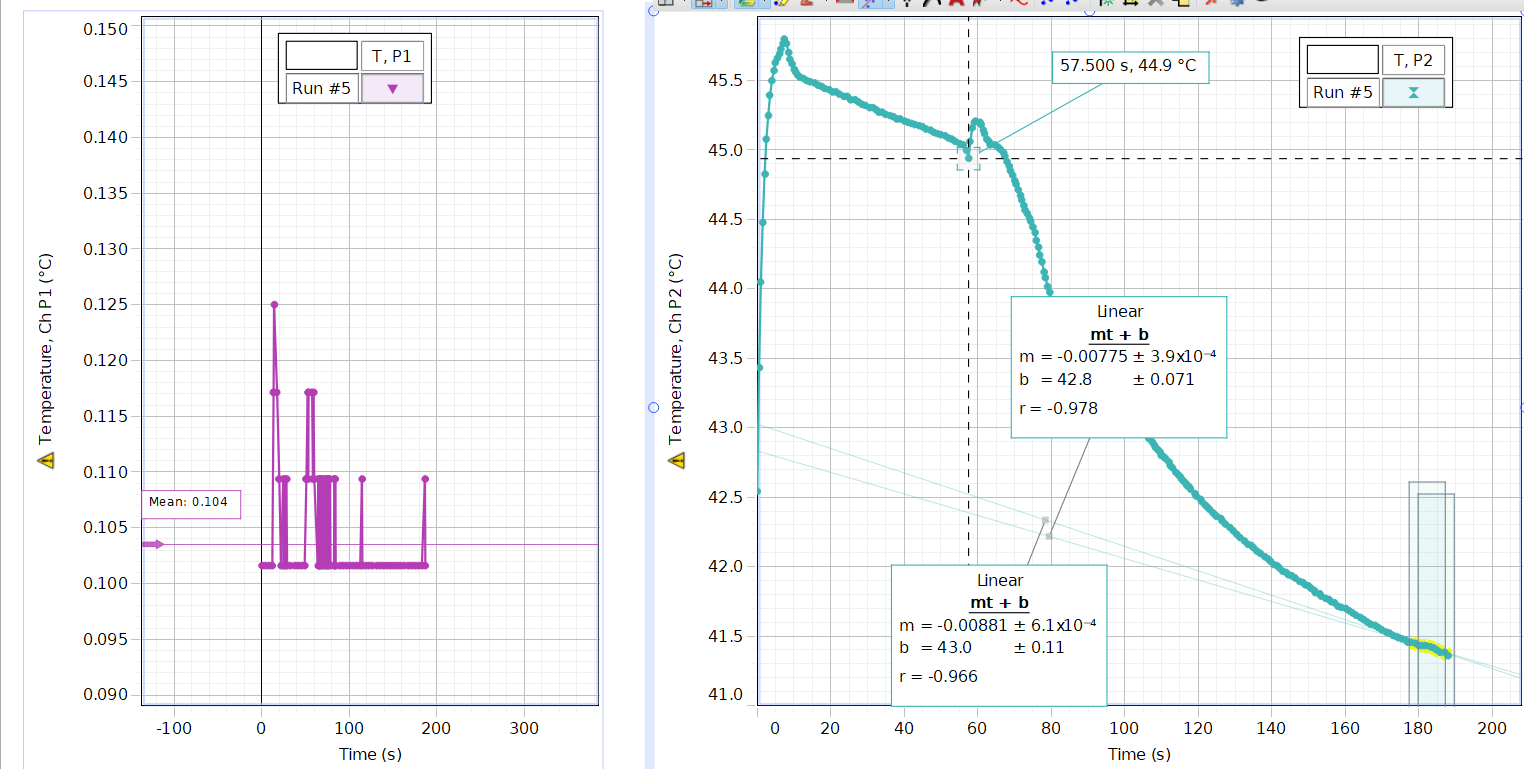
\includegraphics[width=0.9\linewidth]{f3.png}
            \caption{Plot of \(T\) vs \(t\) for metal 3.}
        \end{figure}
    \section{Calculations}
        \begin{equation}
            \begin{split}
                &Q_i = m_ic_i\Delta T_i;~~i = 1, 2, 3\\
                &\Sigma Q_i = 0 \text{ in a calorimeter}\\
                &m_1c_1\Delta T_1 + m_2c_2\Delta T_2 + m_3c_3\Delta T_3 = 0\\
                &T_1 = T_2\\
                &(m_wc_w+m_cc_c)(T_f-T_1) + Mc_M(T_f-T_3) = 0\\
                &c_M = \frac{m_wc_1+m_cc_2}{M}\frac{T_{wi}-T_f}{T_f-T_{mi}}
            \end{split}
        \end{equation}\\[12pt]
        \begin{equation}
            \begin{split}
                \frac{\sigma_{mc}}{\overline{m_c}} &= 0.31\% \\
                T_f &= \frac{T_{fH}+T_{fL}}{2}\\
                T_{f1}&=44.65 \mathrm{\degree C}\\
                T_{f2}&=43.26 \mathrm{\degree C}\\
                T_{f3}&=42.47 \mathrm{\degree C}\\
                \sigma_{Tf}&=\frac{T_{fH}-T_{fL}}{2}\\
                \sigma_{Tf1}&=0.10 \cel\\
                \sigma_{Tf2}&=0.16 \cel\\
                \sigma_{Tf3}&=0.11 \cel\\
                \frac{\sigma_{Tf1}}{T_{f1}} &= 0.23\% \\
                \frac{\sigma_{Tf2}}{T_{f2}} &= 0.25\% \\
                \frac{\sigma_{Tf3}}{T_{f3}} &= 0.43\% \\
            \end{split}
        \end{equation}\\[12pt]
        \begin{equation}
            \begin{split} 
                c_{M1} &= \frac{(0.05725 \text{ kg})(4190~\mathrm{J/(kg\cdot K)})+(0.024787 \text{ kg})(904~\mathrm{J/(kg\cdot K)})}{0.053857 \text{ kg}} \cdot \frac{0.0556 \cel - 44.65 \cel }{44.65 \cel - 48.8 \cel}\\
                &= 453~\mathrm{J/(kg\cdot K)}\\
            \end{split}
        \end{equation}\\[12pt]
        \begin{equation}
            \begin{split}
                c_{M1Tf} &= \frac{(0.05725 \text{ kg})(4190~\mathrm{J/(kg\cdot K)})+(0.024787 \text{ kg})(904~\mathrm{J/(kg\cdot K)})}{0.053857 \text{ kg}} \cdot \frac{ 48.8\cel - 44.66 \cel }{44.44.66 \cel - 0.0556 \cel}\\
                &=463~\mathrm{J/(kg\cdot K)}\\
                \sigma_{cM1} &= \sqrt{(c_{M1Tf} - c_{M1})^2}\\
                &=10 ~\mathrm{J/(kg\cdot K)}\\
            \end{split}
        \end{equation}
    \section{Conclusion}
        The specific heats for metal 1, 2, and 3, were measured to be \(453 \pm 10 ~\mathrm{J/(kg\cdot K)}\), \(886 \pm 50 ~\mathrm{J/(kg\cdot K)}\), and \(289 \pm 12 ~\mathrm{J/(kg\cdot K)}\) respectively. Metal 1 was closest to the specific heat of iron, metal 2 was closest to the specific heat of aluminum, and metal 3 was closest to the specific heat of Bronze. Metal 1 and metal 2 were within a standard deviation of one of the possible metals but metal 3 was not. This is most likely because we stopped the recording for metal 3 too early and the system within the calorimeter had not fully reached equilibrium.
\end{document}